\documentclass{article}
\usepackage{amsmath}
\usepackage{amssymb}
\usepackage{amsthm}
\usepackage{empheq}
\usepackage[most]{tcolorbox}
\usepackage[a4paper, total={6in, 8in}]{geometry}
\usepackage{algorithm}
\usepackage[noend]{algpseudocode}
%\usepackage[francais]{babel}
\usepackage{listings}
\usepackage[utf8]{inputenc}
\usepackage[T1]{fontenc}
\usepackage{subcaption}



\makeatletter
\def\BState{\State\hskip-\ALG@thistlm}
\makeatother

\usepackage{import}
\usepackage{xifthen}
\usepackage{pdfpages}
\usepackage{transparent}
\usepackage{caption}
\usepackage{subcaption}
\usepackage{hyperref}

\captionsetup[subfigure]{labelformat=empty}

\newcommand{\incfig}[1]{%
    \colorbox{white}{
        \def\svgwidth{\columnwidth}
        \import{./figures/}{#1.pdf_tex}
    }
}

\newtheorem{definition}{Definition}
\newtheorem{proposition}{Proposition}
\newtheorem{theorem}{Theorem}
\author{Pierre Glaser, Clement Chadebec}
\title{Rapport de projet - Geodesic Methods and Deformable Models}
\begin{document}
\maketitle
$ \quad $
% \pagebreak
\part{Questions}


\paragraph{Quel est le problème traité} 
Nous étudierons dans ce rapport l'article \emph{Template Matching via densitives on the
Roto Translation Group}, par Erik J. Bekkers et. Al.

Le problème traité est la \textbf{localisation} d'un objet d'intérêt dans une image par
\textbf{apprentissage supervisé}. Dans les jeux de
données utilisés, l'objet est par exemple le disque optique d'un œil, ou bien la
rétine. Le présupposé est que les problèmes en question bénéficieraient d'une prise en
compte des structures d'orientation locale en tout point de l'image.

\paragraph{Quelles sont les équations et les méthodes numériques utilisées} 
\begin{itemize}
    \item La localisation de l'objet d'intérêt se fait par \emph{cross-correlation}: un
        \emph{template} est convolué avec l'image d'intérêt. La valeur maximale du
        résultat est alors la localisation prédite de l'objet. Formellement, si $ f $
        est l'image, et $ x $
    le template:
    \[
        {x}^{\star} = \arg \max_{  } \left ( f \star t \right )(x)
    \] 
    \item Dans le cas standard, $ f $ est définie sur $ \mathbb{R}^2 $. Cependant, $ f $
        peut être transformée (relevée/soulevée?) dans $ \mathbb{R}^3 $, la dimension
        additionnelle décrivant l'état local et l'orientation en tout point d'une image.
    \item Le template final est la solution d'un problème d'optimisation de type
        moindres carrés régularisés, ou régression logistique régularisée.
        Typiquement,
        \[
        t = \arg \min_{  } \sum\limits_{ i=1 }^{ N } \left ( \langle t, p_i \rangle
        - y_i \right )^2 + R(t) 
        \] 
        les $ p_i $ sont des templates individuels: ``idéaux'': ce sont des patches,
        extraits des images, de la même taille que $ t $ centrée en le point d'intérêt
        de l'image $ i $. Si l'on suppose que 
        \begin{itemize}
            \item $ \|p_i\| = 1 $
            \item n'importe quelle coupe de $ f_i $, une image, de la taille de $ p_i $ a une norme
                de $ 1 $
        \end{itemize}
        on a $ (p_i \star f_i)(x) = \mathcal  \langle T_x(p_i) f_i[p_i] \rangle  \leq
        \|p_i\| \|f_i[p_i]\| \leq  1$, le maximum étant atteint quand $ f_i $ et $ p_i $ 
        sont alignés, ceci arrivant par construction en $ {x}^{\star}_i $
        ou $ R $ est une pénalité imposant de la régularité à t.
    \item A ce moment là, le template est une variable dans $ \mathbb{R}^N$, N étant le
        nombre de pixels du patch. On pourrait alors optimiser chaque pixel
        respectivement, mais il serait alors difficile d'imposer des contraintes de
        régularité du patch final. Une autre manière de faire est de paramétriser le
        patch comme une combinaison linéaire de fonctions régulière: c'est l'approche
        suivie dans cet article, qui utilise come fonction les B-splines. Le template
        s'écrit alors
        \[
            t(x, y) = \sum\limits_{ k=1 }^{ N_k } \sum\limits_{ l=1 }^{ N_l } c_{k, l} B^n \left (
            \frac{x}{s_k} - k \right ) B^n \left ( \frac{y}{s_{l}} - l \right )
            \label{eq:spline} \tag{1}
        \] 
        Une expression qui admet alors un gradient, ceci permettant d'ajouter au
        problème d'optimisation un terme de la forme
        \[
            \int\limits_{  }^{  } \| \nabla_{  } t(x, y) \|^2 dx dy
        \] 
\end{itemize}

\paragraph{Pouvez vous situer l'article par rapport aux méthodes étudiées en cours et le
comparer à des sujets proches évoqués en cours} 
La différence principale avec les sujets étudiés en cours est que cette méthode est une
méthode d'apprentissage supervisée et automatique alors que les méthodes étudiées
pendant le cours sont non supervisées et demandent généralement une intervention humaine
au moment de l'initialisation.\newline
Une caractéristique commune de ces deux méthodes est la présence d'un terme de
pénalisation sur la régularité de la solution du problème d'optimisation, les deux
faisant intervenir le gradient le la paramétrisation: on rappelle que le problème des
contours actifs s'écrit:
\[
    \int\limits_{  \Omega }^{  } \left ( w_1^2 \|C'(s)\|^2 + w_2^2 \|C''(s)\|^2 +
    P(C(s)) \right )ds
\] 
alors que le problème étudié concerne la résolution de 
\[
    t = \arg \min_{  } \sum\limits_{ i=1 }^{ N } \left ( \langle t, p_i \rangle
    - y_i \right )^2 + \lambda \int\limits_{  }^{  } \| \nabla_{  } t(x, y) \|^2 dx dy + \mu \| t \|^2
    \label{eq.2} \tag{2}
\]
\paragraph{Quelle est l'originalité du travail (selon les auteurs).} 
Ce travail s'inscrit dans la continuité d'une  série d'article des auteurs: la majorité
des concepts utilisés dans cet articles on été introduits dans des publications
précédentes:
\begin{itemize}
    \item l'utilisation des scores d'orientation a été introduit en [32]
    \item l'utilisation des cake wavelets a été introduit dans la thèse de l'auteur.
    \item la cross correlation est une technique bien connue pour détecter des points
        d'intérêts.
\end{itemize}
Les auteurs proposent alors une méthode de résolution pour une reformulation de la 
``regression logistique'' permettant à cette méthode d'atteindre l'état de l'art en
termes de performances, ainsi qu'une série d'expériences très completes
comparant l'influence des différents types de régularisation et l'importance des
orientation scores. Enfin, est donnée en appendice une interprétation mathématique d'une
version simplifiée du problème régularisé dans $ SE2(\mathbb{R}) $
\paragraph{Quels sont les résultats nouveaux importants qui en découlent.}
Le résultat le plus important ici est à nos yeux la preuve expérimentale que cette
méthode atteint l'état de l'art pour les jeux de données considérées.
\paragraph{Voyez vous des faiblesses dans l'approche présentée et avez-vous des idées
pour y faire face?}

\part{Rapport détaillé}
\section{Discussions théoriques}
\paragraph{Les scores d'orientation} 
Un concept majeur du papier concerne la manière de prendre en compte les l'état
d'orientation de chaque point de l'image afin de mieux détecter le point d'intérêt.
L'approche consiste a convoluer l'image avec le $ R_{\theta} w $, ou $ R_{\theta} $ est la rotation d'angle $ \theta  $, et $ w $ est une ondelette.
l'image 
\[
    \begin{aligned}
        f: \mathbb{R}^2 &\longrightarrow \mathbb{R} \\
        (x, y) &\longmapsto f(x, y)
    \end{aligned}
\] 
devient alors 
\[
\begin{aligned}
    U_f: \quad \mathbb{R}^2\times \mathbb{ T } &\longrightarrow \mathbb{R} \\
    (x, y, \theta) &\longmapsto g(x, y, \theta)
\end{aligned}
\] 
$ \theta $, tout comme $ x $ et $ y $ est discrétisé.
La construction de ce score d'orientation est inspirée par le fonctionnement du cortex
visuel des mammifères (voir \emph{Image Analysisand Reconstruction using a Wavelet
Transform constructed from a Reducible Representation of the Euclidean Motion Group}).
On effectue alors un certain nombres de remarques sur cette transformée
\begin{itemize}
    \item Par definition, $  U_f $ est une transformée en ondelettes:
        \[
             U_f(g) =  (\mathcal W_{\phi}[f])(g)  = \langle \mathcal  U_g \phi, f
             \rangle_{\mathbb{R}^2}
        \] 
        et $ \mathcal  U_g $ est une representation:
        \[
            \mathcal  U_g \phi(x) = (\mathcal  T_b \mathcal  R_{e^{i \theta}} \phi )(x)
            = \phi \left ( R_{\theta}^{-1}(x - b) \right )
        \] 
        \item $ f  \to U_f $ transforme $ L_2(\mathbb{R}) $ en un espace de Hilbert $
        \mathbb C_K^{\mathbb{R}^2 \times \mathbb{ T }} $.\newline
        Tout comme la transformée de Fourier (aux constantes multiplicatives près), la
        transformation $ U_f $ est une isométrie:
        \[
            \|f\|_{L_2(\mathbb{R})} = \|U_f\|_{M_{\phi}}
        \] 
        où $ M_{\phi} $ est une fonction caractérisant le produit scalaire de cet espace
        de Hilbert.\newline
        De cette propriété découle l'inversibilité de la transformée en scores
        d'orientations.
        \item contrairement à la transformée en ondelettes classique, cette transformée
            ne fait pas intervenir différentes échelles, ce qui dans les cas étudiés,
            semble être considéré comme quelque chose de désirable.
        \item la stabilité de la transformée inverse est complètement déterminée par la
            fonction $ M_{\phi} $, et donc (évidemment), et c'est sous ce critère que la
            l'ondelette de base $ \phi $ est choisie.
\end{itemize}
Les ondelettes ``cake'' (gateau en anglais) s'avèrent avoir un $ M_{\phi} $ optimal, et
être d'excellents détecteurs de lignes. C'est donc cette ondelette qui a été choisie
comme base pour créer les scores d'orientation dans le papier étudié.
\begin{figure}[htpb]
\centering
\hspace*{-6em}
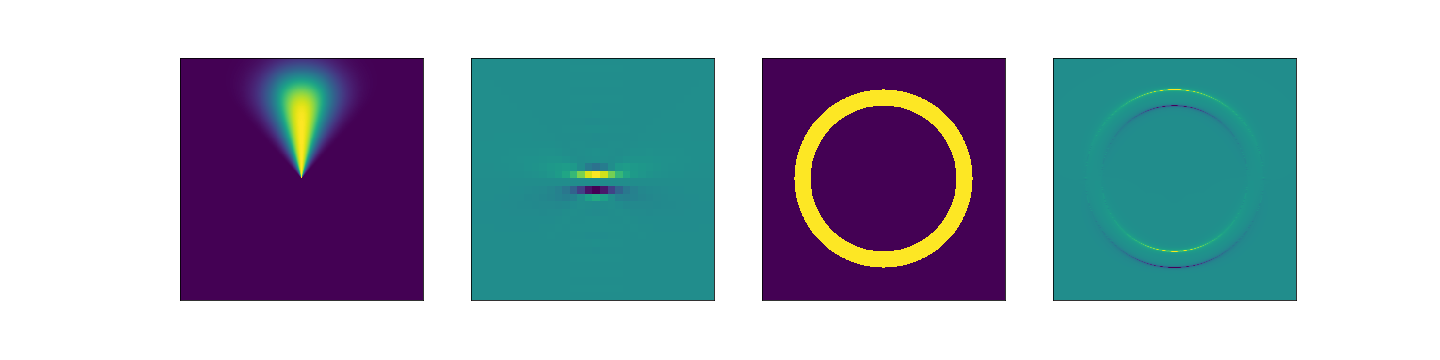
\includegraphics[scale=0.39]{plots/cake_wavelet.png}
\caption {Simulation personnelles des ondelettes de  cake}
de gauche à droite: l'ondelette dans le plan de fourrier, l'ondelette dans le domaine
spatial, une image simple, et la même image transformée par cette ondelette.
\end{figure}

\paragraph{Extension à $SE(2)$}
Comme présenté au dessus, le score d'orientation permet de capturer d'une certaine manière les axes dominants d'un image dans une certaine direction. De ce fait, 
l'utilisation de ce score semble être d'intérêt pour des problèmes de détection.
Dans, ce papier les auteurs ont ainsi fait le choix d'étendre le problème d'optimisation comme présenté en \ref{eq.2} à $SE(2)$ via 
l'utilisation du score d'orientation. Il s'agit désormais de s'intéresser au problème d'optimisation étendu:
\[
  \sum \limits_{i=1}^N (\langle t, |U_{fi}| \rangle_{{\mathbb{L}_2(SE(2))}} - y_i)^2 + \lambda \int \limits_{\mathbb{R}^2} \int \limits_{0}^{2\pi} \lVert 
  \nabla t(x, y, \theta)\rVert_{D}^2 dxdyd\theta + \mu \lVert t \rVert_{\mathbb{L}_2(SE(2))}^2
\]
Les $U_{fi}$ sont les scores d'orientation des patchs ``idéaux'' $p_i$.
Le produit scalaire définit sur $SE(2)$ prend la forme suivante:
\[
    \langle t, |U_{fi}| \rangle_{SE(2)} = 
    \int \limits_{\mathbb{R}^2} \int \limits_{0}^{2\pi} \overline{t(x, y, \theta)} \lvert U_f (x, y, \theta) \rvert dxdyd\theta
\]

Et $\nabla t$ est le gradient invariant à gauche déduit des dérivées partielles invariantes à gauches définies sur $SE(2)$
comme suit $\{\partial_{\xi} = cos(\theta)\partial_x + sin(\theta) \partial_y,\, \partial{\eta} = -sin(\theta) \partial_x + cos(\theta)
\partial_y, \partial_{\theta}\}$. Le gradient est alors déduit:
\[
    \lVert \nabla t \rVert_{D}^2 = D_{\xi \xi} \Big|\frac{\partial t}{\partial \xi} \Big|^2
    + D_{\eta \eta} \Big|\frac{\partial t}{\partial \eta}\Big|^2 + D_{\theta \theta} \Big|\frac{\partial t}{\partial \theta}\Big|^2
\]
\textcolor{red}{C'est quoi $ D_{ \xi \xi}, D_{\eta \eta}  $ etc.?}


De manière identique à l'approche employée dans $\mathbb{R}^2$, le template final est paramétré par une famille de fonctions
régulières telles que les B-splines étendues à $SE(2)$
\[
    t(x, y, \theta) = \sum \limits_{k=1}^{n_k} \sum \limits_{l=i}^{N_l} \sum \limits_{m=1}^{N_m} c_{k,l,m} B^n \left (\frac{x}{s_k} - k \right )
    B^n \left (\frac{y}{s_l} - l \right) B^n \left (\frac{\theta \text{mod} 2\pi}{s_m} - m \right )
\]

\paragraph{Regression logistique}
Dans les deux espaces considérés, $\mathbb{R}^2$ et $SE(2)$, un modèle de regression logistique est également proposé en comparaison 
au modèle de régression linéaire. Dans les problèmes de détection, le but majeur est de séparer les patches $f_i$ correspondant aux zones d'une image correspondant à une 
zone d'intérêt ($y_i =1$) des zones sans objet ($y_1=0$). Cependant, une approche différente de \ref{eq.2} et ne faisant pas intervenir le terme de perte quadratique 
peut être également employée. Ici, les auteurs ont décidé d'avoir recours à un modèle de régression logistique dans lequel la présence ou non de 
la zone d'intérêt au sein d'un patch $f_i$ est représentée par une certaine probabilité de présence $p_i$. Cette probabilité est inférée à l'aide de
la function ``sigmoide'' telle que $p_i = \sigma(\langle t, f_i \rangle)$. Le le but revient à trouver le template qui maximise la vraisemblance $l(t) = 
\prod \limits_{i=1}^N p(f_i; t)^{y_i}(1 - p(f_i; y))^{1- y_i}$
des patches $f_i$ étant donnés leurs labels $y_i$. Dans une telle approche la log-vraissemenblance permet de 'linéariser' le problème d'optimisation qui prend la forme
suivante dans $\mathbb{R}^2$:
\[
    \arg \max \sum \limits_{i=1}^N \langle t, f_i \rangle_{\mathbb{L}_2(\mathbb{R}^2)} - \log \left ( 1 + e^{\langle t, f_i \rangle_{\mathbb{L}_2(\mathbb{R}^2)}}\right) - \lambda \int \limits_{\mathbb{R}^2} \lVert \nabla 
    t \rVert_{\mathbb{L}_2(\mathbb{R}^2)}^2 dx dy - \mu \lVert t \rVert_{\mathbb{L}_2(\mathbb{R}^2)}^2
\]
ou dans $SE(2)$:
\[
    \arg \max \sum \limits_{i=1}^N \langle t, |U_{f_i}| \rangle_{\mathbb{L}_2(SE(2))} - \log \left ( 1 + e^{\langle t, |U_{f_i}| \rangle_{\mathbb{L}_2(SE(2))}}\right) - \lambda \int \limits_{\mathbb{R}^2} \int \limits_{0}^{2\pi}\lVert \nabla 
    t \rVert_{D}^2 dx dy d\theta- \mu \lVert t \rVert_{\mathbb{L}_2(SE(2))}^2
\]



\section{Expériences}

Afin de mieux comprendre leur fonctionnement et de pouvoir les comparer dans 
divers cadres d'études, nous avons re-codé les différentes méthodes présentées dans cet article 
en langage \textit{python}. Le code complet peut être trouvé au lien suivant ???????
Pour mémoire, 5 types de construction de templates sont envisagés:
\begin{itemize}
    \item A: Template obtenu par moyenne de tous les patches positifs (i.e. centrés sur la zone d'intérêt) et normalisation.
    \item B: Template optimisé sans régularisation ($\mu =0$, $\lambda = 0$)
    \item C: Template optimisé avec $\mu$ ($\lambda=0$)
    \item D: Template optimisé avec $\lambda$ ($\mu = 0$)
    \item E: Template optimisé avec $\mu$ et $\lambda$
\end{itemize}

Pour chacune de ses constructions, un module de regression linéaire et regression logistique est employé dans 
les espaces $\mathbb{R}^2$ et $SE(2)$. Afin de réaliser les expérience dont les résultats sont présentés plus 
ont été réalisée en considérant un ensemble de 500 images dont 80\% (400 images) constitue l'ensemble d'entrainement 
des modèles et les 20 \% (100 images) restants l'ensemble de test. Sur chacune des images d'entrainement, un patch 
positif de taille $N_x \times N_y = 101 \times 101$ centré autour des coordonnées de l'œil gauche et un patch négatif 
de même de taille tiré aléatoirement en dehors des zones d'intérêts (œil droit et gauche) sont crées. Une détection est 
ensuite considérée "bonne" sur le point de détection se situe dans rayon de $10$ pixels autour de la position réelle de l'œil 
gauche. Le nombre de splines considéré est de $N_k = 51$ , $N_l =51$ et $N_m = 4$.



\paragraph{Template Matching dans $\mathbb{R}^2$}
Premièrement, une comparaison des résultats obtenus avec les différentes méthodes a été réalisée dans $\mathbb{R}^2$.
Les résultats sont reportés dans \ref{table: R2}. Afin de trouver les valeurs optimales de $\mu$ (resp $\lambda$) dans les expériences C (resp. D), nous avons décidé 
de procéder de façon empirique en faisant varier les valeurs de ces deux paramètres entre $10^{-4}$ et $1$. Afin de trouver le meilleur couple pour l'expérience E, nous avons 
choisi de tout d'abord fixer la valeur de $\mu$ et $\lambda$ à leur valeur optimale
trouvée lors des expériences C et D $ {\mu}^{\star}$ et $ {\lambda}^{\star}$, puis de faire légèrement leurs valeurs autour de ces optimaux.
Il s'est avéré que comme présenté dans l'article un choix de couple $\mu = 0.5
{\mu}^{\star}$ et $\lambda = 0.5 {\lambda}^{\star}$ fournissait les meilleurs résultats.

\begin{table}[h!]
    \centering
    \begin{tabular}{|c|c|c|}
        \hline
        Méthode & Score (\%)\\
        \hline
        \hline
        $A^{\mathbb{R}^2}$& 61.0 \% \\
        \hline
        $B_{\text{lin}}^{\mathbb{R}^2}$& 3.0 \%    \\
        $C_{\text{lin}}^{\mathbb{R}^2}$& 62.0 \%   \\
        $D_{\text{lin}}^{\mathbb{R}^2}$& 38.0 \%   \\
        $E_{\text{lin}}^{\mathbb{R}^2}$& 62.0 \%   \\
        \hline
        $B_{\text{log}}^{\mathbb{R}^2} $& 0.0 \%   \\ 
        $C_{\text{log}}^{\mathbb{R}^2} $& 63.0 \%  \\ 
        $D_{\text{log}}^{\mathbb{R}^2} $& 26.0 \%   \\ 
        $E_{\text{log}}^{\mathbb{R}^2} $& 63.0 \%  \\ 
        \hline
    \end{tabular}
    \caption{Résultats obtenus par template matching dans $\mathbb{R}^2$}
    \label{table: R2}
\end{table}

La table \ref{table: R2} montre qu'un template relativement simple ne correspondant finalement qu'à la moyenne de tous les patches positifs démontre tout de même de bons
résultats comparé à des modèles de régression plus évolués. Effectivement, si non couplés à de mécanismes de régularisation, les modèles $B_{\text{log}}^{\mathbb{R}^2} $ et 
$B_{\text{lin}}^{\mathbb{R}^2} $ ne démontre que de faibles performances. Par ailleurs, un bon choix de paramètres de régularisation peut conduire à améliorer drastiquement les 
performances des regressions dont le meilleur résultat est observé pour $\mu = 10^{-1}$ et $\lambda = 10^{-2}$ pour la regression linéaire et $\mu = 10^{-1}$ et $\lambda = 10^{-3}$ pour la regression logistique.
C'est deux modèles de regression semblent d'ailleurs démontrer des niveaux de performance similaire.
Le "meilleur" modèle dans $\mathbb{R}^2$ est néanmoins obtenu dans le cas E avec la regression logistique (63\%). Ces résultats semblent alignés avec ceux présentés par les auteurs bien que dans $\mathbb{R}^2$, 
il semble que le patch moyenné $A^{\mathbb{R}^2}$ démontre les meilleurs résultats, les
suivant sont $C_{\text{lin}}^{\mathbb{R}^2}, E_{\text{lin}}^{\mathbb{R}^2},
C_{\text{lin}}^{\mathbb{R}^2}$ et $E_{\text{log}}^{\mathbb{R}^2}$ qui marchent de manière 
similaires.


\paragraph{Template Matching dans $SE(2)$}
Les mêmes expériences ont ensuite été reproduites en utilisant l'espace $SE(2)$ et donc ajoutant également l'orientation score dans les régressions.
Cependant, dans cette section les paramètres le paramètres $\mu \in [10^{-5}, 10^{-1}]$ et $\lambda \in [10^{-4}, 10^{-1}]$. En ce qui concernent les paramètres inhérents à la matrices de 
régularisation ont été fixé comme suit $D_{\xi \xi}=1, D_{\eta \eta} = 0$ et $D_{\theta \theta} = 10^{-2}$. Nous n'avons pas fait varié ces paramètres qui ont été choisis en accord avec les auteurs 
de l'article présenté. Les résultats peuvent être observés en \ref{table: SE(2)}.

\begin{table}[h!]
    \centering
    \begin{tabular}{|c|c|c|}
        \hline
        Méthode & Score (\%)\\
        \hline
        \hline
        $A^{SE(2)}$&  63.0 \% \\
        \hline
        $B_{\text{lin}}^{SE(2)}$&  67.0    \%   \\
        $C_{\text{lin}}^{SE(2)}$&  88.0    \%   \\
        $D_{\text{lin}}^{SE(2)}$&  26.0   \%   \\
        $E_{\text{lin}}^{SE(2)}$&  89.0    \%   \\
        \hline
        $B_{\text{log}}^{SE(2)} $&  7.0  \%   \\ 
        $C_{\text{log}}^{SE(2)} $&  55.0  \%   \\ 
        $D_{\text{log}}^{SE(2)} $&  18.0 \%   \\ 
        $E_{\text{log}}^{SE(2)} $&  53.0  \%   \\ 
        \hline
    \end{tabular}
    \caption{Résultats obtenus par template matching dans $SE(2)$}
    \label{table: SE(2)}
\end{table}

Finalement, les résultats présentés en \ref{table: SE(2)} démontrent l'intérêt de considérer des templates dans un espace étendu tel que $SE(2)$.
Si le template créé par moyenne de tous les patches positifs ne marche que légèrement mieux dans $SE(2)$ (63\% v. 61\%), l'efficacité 
lors de la création de template via des régressions dans $SE(2)$ est remarquable. En effet, une simple régression linéaire sans aucune régularisation permet 
d'atteindre un niveau de performance bien supérieur passant de 3\% dans $\mathbb{R}^2$ à 67\% dans $SE(2)$. Si maintenant, 
un simple régularisation $l-2$ est considérée (cas C), combinée à un choix judicieux de $\mu$,  la performance peut atteindre 88\% de précision.
L'ajout d'un nouveau terme régularisant (cas E) et un bon choix de constante permet d'obtenir le meilleur résultat. Seul le cas D, démontre une 
performance plus faible que le même cas dans $\mathbb{R}^2$ qui était également l'un des moins performants. Les résultats que nous présentons sont en ligne avec ceux 
présentés par les auteurs en ce qui concerne les regressions linéaires. Notre meilleur modèle est dérivé de la méthode $C_{\text{lin}}^{SE(2)}$. Pour 
les regressions logistiques, nos résultats sont un peut décevants en comparaison de ceux présenté par les auteurs. 



\begin{figure*}[h!]
    \centering

    \begin{subfigure}[b]{0.3\textwidth}
        \centering
        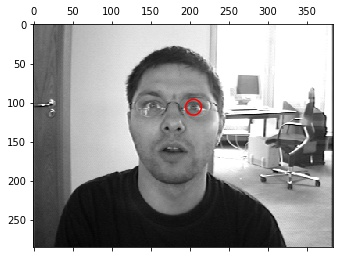
\includegraphics[width=\textwidth]{plots/test_image_detection.jpg}
        \caption{test image}
    \end{subfigure}

    {\small (a)}

    \vskip\baselineskip
    \begin{subfigure}[b]{0.1\textwidth}
        \centering
        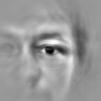
\includegraphics[width=\textwidth]{plots/A_R2_template.jpg}

    \end{subfigure}
    \hspace{-1\baselineskip}
    \vspace{-0.5\baselineskip}
    \quad
    \begin{subfigure}[b]{0.1\textwidth}  
        \centering 
        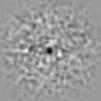
\includegraphics[width=\textwidth]{plots/B_lin_R2_template.jpg}

    \end{subfigure}
    \hspace{-1\baselineskip}
    \quad
    \begin{subfigure}[b]{0.1\textwidth}   
        \centering 
        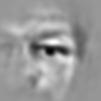
\includegraphics[width=\textwidth]{plots/C_lin_R2_template.jpg}

    \end{subfigure}
    \hspace{-1\baselineskip}
    \quad
    \begin{subfigure}[b]{0.1\textwidth}   
        \centering 
        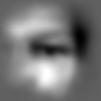
\includegraphics[width=\textwidth]{plots/D_lin_R2_template.jpg}

    \end{subfigure}
    \hspace{-1\baselineskip}
    \quad
    \begin{subfigure}[b]{0.1\textwidth}   
        \centering 
        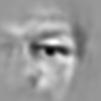
\includegraphics[width=\textwidth]{plots/E_lin_R2_template.jpg}

    \end{subfigure}
    \hspace{-1\baselineskip}
    \quad
    \begin{subfigure}[b]{0.1\textwidth}   
        \centering 
        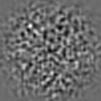
\includegraphics[width=\textwidth]{plots/B_log_R2_template.jpg}

    \end{subfigure}
    \hspace{-1\baselineskip}
    \quad
    \begin{subfigure}[b]{0.1\textwidth}   
        \centering 
        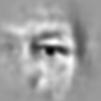
\includegraphics[width=\textwidth]{plots/C_log_R2_template.jpg}

    \end{subfigure}
    \hspace{-1\baselineskip}
    \quad
    \begin{subfigure}[b]{0.1\textwidth}   
        \centering 
        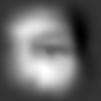
\includegraphics[width=\textwidth]{plots/D_log_R2_template.jpg}

    \end{subfigure}
    \hspace{-1\baselineskip}
    \quad
    \begin{subfigure}[b]{0.1\textwidth}   
        \centering 
        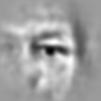
\includegraphics[width=\textwidth]{plots/E_log_R2_template.jpg}

    \end{subfigure}
    \vskip\baselineskip
    \begin{subfigure}[b]{0.1\textwidth}
        \centering
        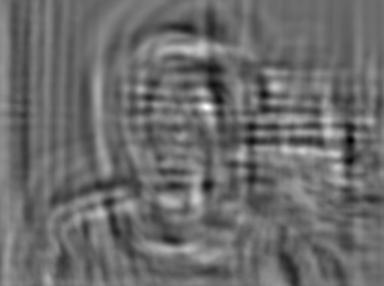
\includegraphics[width=\textwidth]{plots/A_R2_conv.jpg}
        \caption{$A^{\mathbb{R}^2}$}%
        
        \label{fig:mean and std of net14}
    \end{subfigure}
    \hspace{-1\baselineskip}
    \quad
    \begin{subfigure}[b]{0.1\textwidth}  
        \centering 
        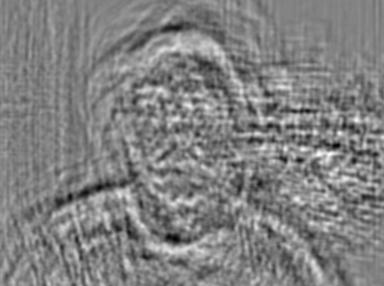
\includegraphics[width=\textwidth]{plots/B_lin_R2_conv.jpg}
        \caption{$B_{\text{lin}}^{\mathbb{R}^2}$}%
         
        \label{fig:mean and std of net24}
    \end{subfigure}
    \hspace{-1\baselineskip}
    \quad
    \begin{subfigure}[b]{0.1\textwidth}   
        \centering 
        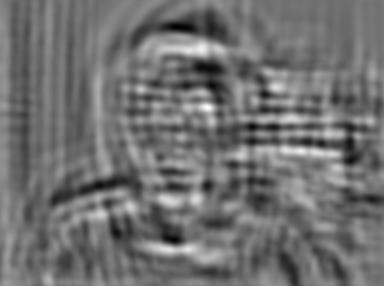
\includegraphics[width=\textwidth]{plots/C_lin_R2_conv.jpg}
        \caption{$C_{\text{lin}}^{\mathbb{R}^2}$}%
           
        \label{fig:mean and std of net34}
    \end{subfigure}
    \hspace{-1\baselineskip}
    \quad
    \begin{subfigure}[b]{0.1\textwidth}   
        \centering 
        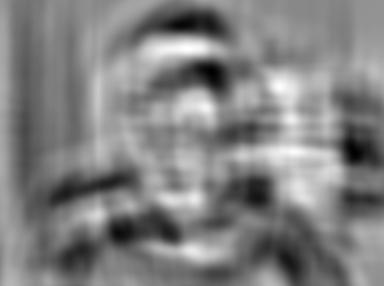
\includegraphics[width=\textwidth]{plots/D_lin_R2_conv.jpg}
        \caption{$D_{\text{lin}}^{\mathbb{R}^2}$}%
        
        \label{fig:mean and std of net44}
    \end{subfigure}
    \hspace{-1\baselineskip}
    \quad
    \begin{subfigure}[b]{0.1\textwidth}   
        \centering 
        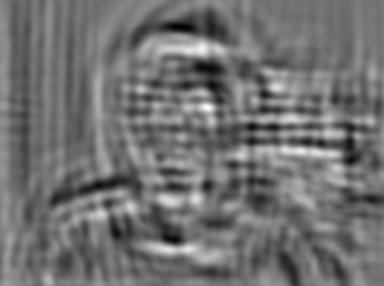
\includegraphics[width=\textwidth]{plots/E_lin_R2_conv.jpg}
        \caption{$E_{\text{lin}}^{\mathbb{R}^2}$}%
        
        \label{fig:mean and std of net44}
    \end{subfigure}
    \hspace{-1\baselineskip}
    \quad
    \begin{subfigure}[b]{0.1\textwidth}   
        \centering 
        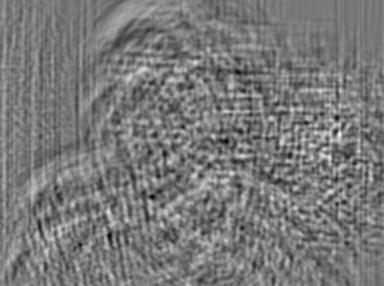
\includegraphics[width=\textwidth]{plots/B_log_R2_conv.jpg}
        \caption{$B_{\text{log}}^{\mathbb{R}^2}$}%
        
        \label{fig:mean and std of net44}
    \end{subfigure}
    \hspace{-1\baselineskip}
    \quad
    \begin{subfigure}[b]{0.1\textwidth}   
        \centering 
        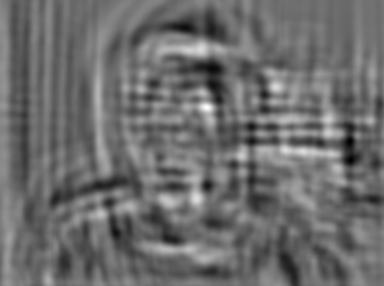
\includegraphics[width=\textwidth]{plots/C_log_R2_conv.jpg}
        \caption{$C_{\text{log}}^{\mathbb{R}^2}$}%
        
        \label{fig:mean and std of net44}
    \end{subfigure}
    \hspace{-1\baselineskip}
    \quad
    \begin{subfigure}[b]{0.1\textwidth}   
        \centering 
        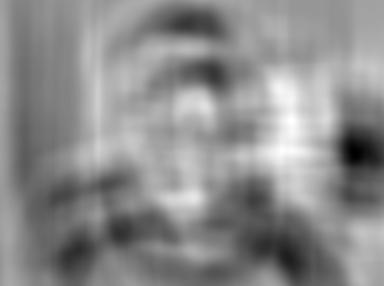
\includegraphics[width=\textwidth]{plots/D_log_R2_conv.jpg}
        \caption{$D_{\text{log}}^{\mathbb{R}^2}$}%
        
        \label{fig:mean and std of net44}
    \end{subfigure}
    \hspace{-1\baselineskip}
    \quad
    \begin{subfigure}[b]{0.1\textwidth}   
        \centering 
        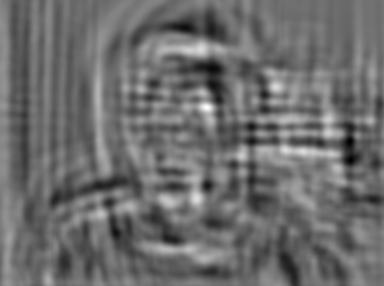
\includegraphics[width=\textwidth]{plots/E_log_R2_conv.jpg}
        \caption{$E_{\text{log}}^{\mathbb{R}^2}$}%
        
        \label{fig:mean and std of net44}
    \end{subfigure}
    {\small (a)}
    \vskip\baselineskip
    \begin{subfigure}[b]{0.1\textwidth}
        \centering
        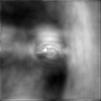
\includegraphics[width=\textwidth]{plots/A_SE2_template.jpg}

    \end{subfigure}
    \hspace{-1\baselineskip}
    \vspace{-0.5\baselineskip}
    \quad
    \begin{subfigure}[b]{0.1\textwidth}  
        \centering 
        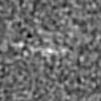
\includegraphics[width=\textwidth]{plots/B_lin_SE2_template.jpg}

    \end{subfigure}
    \hspace{-1\baselineskip}
    \quad
    \begin{subfigure}[b]{0.1\textwidth}   
        \centering 
        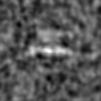
\includegraphics[width=\textwidth]{plots/C_lin_SE2_template.jpg}

    \end{subfigure}
    \hspace{-1\baselineskip}
    \quad
    \begin{subfigure}[b]{0.1\textwidth}   
        \centering 
        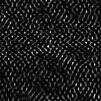
\includegraphics[width=\textwidth]{plots/D_lin_SE2_template.jpg}

    \end{subfigure}
    \hspace{-1\baselineskip}
    \quad
    \begin{subfigure}[b]{0.1\textwidth}   
        \centering 
        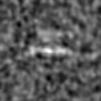
\includegraphics[width=\textwidth]{plots/E_lin_SE2_template.jpg}

    \end{subfigure}
    \hspace{-1\baselineskip}
    \quad
    \begin{subfigure}[b]{0.1\textwidth}   
        \centering 
        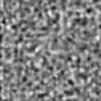
\includegraphics[width=\textwidth]{plots/B_log_SE2_template.jpg}

    \end{subfigure}
    \hspace{-1\baselineskip}
    \quad
    \begin{subfigure}[b]{0.1\textwidth}   
        \centering 
        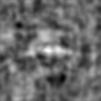
\includegraphics[width=\textwidth]{plots/C_log_SE2_template.jpg}

    \end{subfigure}
    \hspace{-1\baselineskip}
    \quad
    \begin{subfigure}[b]{0.1\textwidth}   
        \centering 
        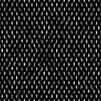
\includegraphics[width=\textwidth]{plots/D_log_SE2_template.jpg}

    \end{subfigure}
    \hspace{-1\baselineskip}
    \quad
    \begin{subfigure}[b]{0.1\textwidth}   
        \centering 
        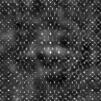
\includegraphics[width=\textwidth]{plots/E_log_SE2_template.jpg}

    \end{subfigure}
    \vskip\baselineskip
    \begin{subfigure}[b]{0.1\textwidth}
        \centering
        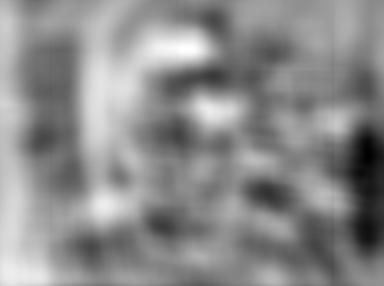
\includegraphics[width=\textwidth]{plots/A_SE2_conv.jpg}
        \caption{$A^{SE(2)}$}%
        
        \label{fig:mean and std of net14}
    \end{subfigure}
    \hspace{-1\baselineskip}
    \quad
    \begin{subfigure}[b]{0.1\textwidth}  
        \centering 
        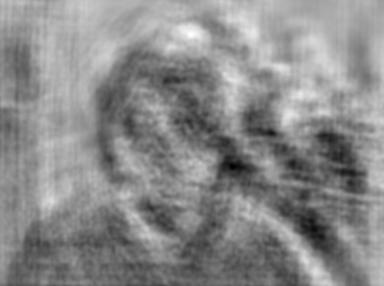
\includegraphics[width=\textwidth]{plots/B_lin_SE2_conv.jpg}
        \caption{$B_{\text{lin}}^{SE(2)}$}%
         
        \label{fig:mean and std of net24}
    \end{subfigure}
    \hspace{-1\baselineskip}
    \quad
    \begin{subfigure}[b]{0.1\textwidth}   
        \centering 
        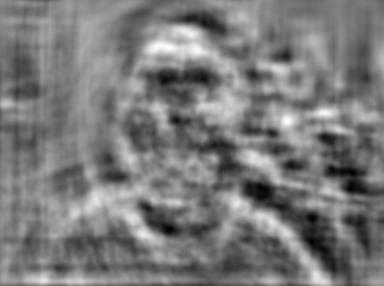
\includegraphics[width=\textwidth]{plots/C_lin_SE2_conv.jpg}
        \caption{$C_{\text{lin}}^{SE(2)}$}%
           
        \label{fig:mean and std of net34}
    \end{subfigure}
    \hspace{-1\baselineskip}
    \quad
    \begin{subfigure}[b]{0.1\textwidth}   
        \centering 
        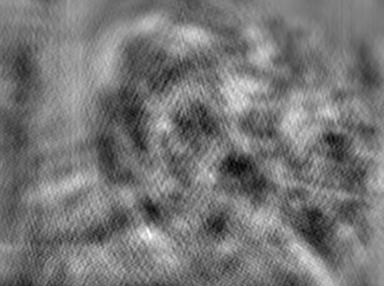
\includegraphics[width=\textwidth]{plots/D_lin_SE2_conv.jpg}
        \caption{$D_{\text{lin}}^{SE(2)}$}%
        
        \label{fig:mean and std of net44}
    \end{subfigure}
    \hspace{-1\baselineskip}
    \quad
    \begin{subfigure}[b]{0.1\textwidth}   
        \centering 
        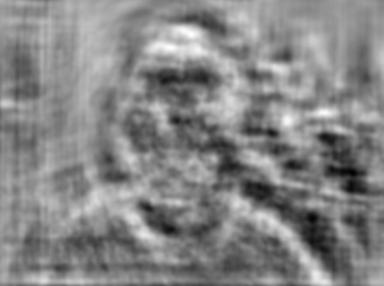
\includegraphics[width=\textwidth]{plots/E_lin_SE2_conv.jpg}
        \caption{$E_{\text{lin}}^{SE(2)}$}%
        
        \label{fig:mean and std of net44}
    \end{subfigure}
    \hspace{-1\baselineskip}
    \quad
    \begin{subfigure}[b]{0.1\textwidth}   
        \centering 
        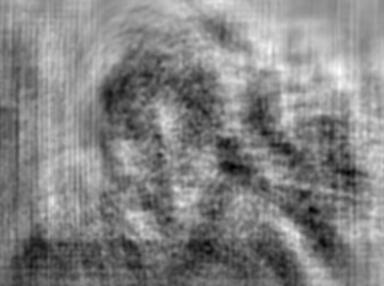
\includegraphics[width=\textwidth]{plots/B_log_SE2_conv.jpg}
        \caption{$B_{\text{log}}^{SE(2)}$}%
        
        \label{fig:mean and std of net44}
    \end{subfigure}
    \hspace{-1\baselineskip}
    \quad
    \begin{subfigure}[b]{0.1\textwidth}   
        \centering 
        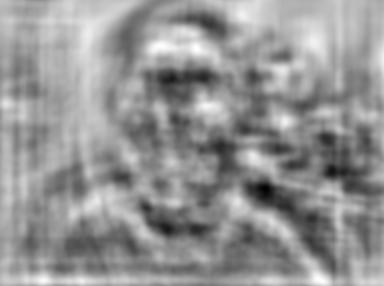
\includegraphics[width=\textwidth]{plots/C_log_SE2_conv.jpg}
        \caption{$C_{\text{log}}^{SE(2)}$}%
        
        \label{fig:mean and std of net44}
    \end{subfigure}
    \hspace{-1\baselineskip}
    \quad
    \begin{subfigure}[b]{0.1\textwidth}   
        \centering 
        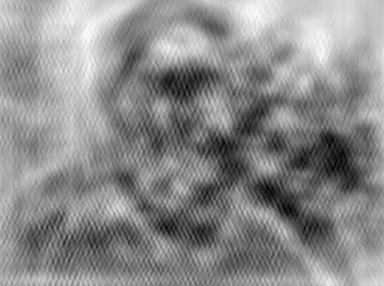
\includegraphics[width=\textwidth]{plots/D_log_SE2_conv.jpg}
        \caption{$D_{\text{log}}^{SE(2)}$}%
        
        \label{fig:mean and std of net44}
    \end{subfigure}
    \hspace{-1\baselineskip}
    \quad
    \begin{subfigure}[b]{0.1\textwidth}   
        \centering 
        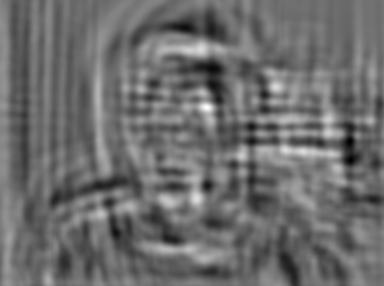
\includegraphics[width=\textwidth]{plots/E_log_R2_conv.jpg}
        \caption{$D_{\text{log}}^{SE(2)}$}%
        
        \label{fig:mean and std of net44}
    \end{subfigure}

    {\small (b)}

    \caption[ The average and standard deviation of critical parameters ]
    {\small Exemples de templates et leur réponse} 
    \label{fig: template}
\end{figure*}

La figure \ref{fig: template} représente (a) l'image test (b) les différents templates de $\mathbb{R}^2$ que nous avons obtenus sur la première ligne ainsi que leur réponse dans les différents 
cas considérés sur la seconde ligne (b) le maximum d'intensité du template à travers les orientations $\theta$ ainsi que la réponse du template à l'image test.

\paragraph{Influence de la régularisation}

Nous avons voulu rendre compte de l'influence des différents paramètres de régularisation sur la précision du modèle.
Pour ce faire nous avons reporté les valeurs de précision des modèles $C_{\text{lin}}^{SE(2)}$ et $D_{\text{lin}}^{SE(2)}$
en faisant varier les valeurs de $\mu$ et $\lambda$. Les résultats sont visibles en \ref{fig:param}. Cette courbe permet de bien rendre 
compte de l'importance de la régularisation dans un tel problème de détection.

\paragraph{Influence du critère de précision}
Afin d'être tout à fait transparents sur la précision des modèles développé nous avons testé le modèle démontrant les meilleurs 
résultats $C_{\text{lin}}^{SE(2)}$ avec différents valeur de rayon de détection variant de $2$ pixels à $50$ pixels. Les résultats 
peuvent être appréciés en \ref{fig:radius}. Pour un rayon de détection de 2 pixels, la précision du modèle tombe à $37 \%$. Ceci n'est pas 
étonnant dans la mesure où 2 pixels rentre largement dans la gamme de précision de ``labélisation''. Par contre, pour un rayon de détection de 5 pixels, 
le modèle démontre une précision assez bonne de 81 \%, ce qui est en lien avec la valeur précédemment observée pour 10 pixels. Dés que le rayon dépasse 
15 pixels, la précision du modèle stagne. Ceci laisse apercevoir que 10\% des détections sont aberrantes.

\begin{figure}[htpb]
\centering
\hspace*{-5em}%
\begin{subfigure}{.6\textwidth}
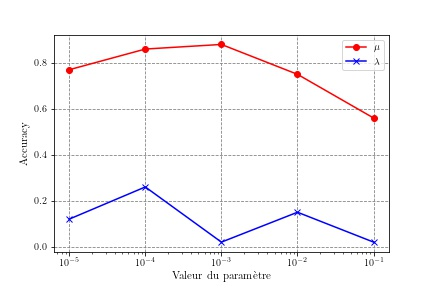
\includegraphics[scale=0.65]{plots/parameter_score_C_D_lin_R2.jpg}%
  \caption{$ \quad \quad \quad $Influence des paramètres de régularisation}%
    \label{fig:param}
\end{subfigure}%
%\hspace*{5em}
\begin{subfigure}{.6\textwidth}
  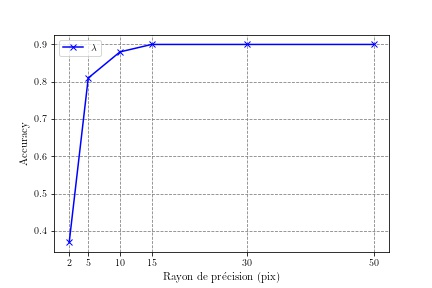
\includegraphics[scale=0.65]{plots/radius_scores.jpg}
  \caption{ Précision en fonction du rayon de détection}%
  \label{fig:radius}
\end{subfigure}
\end{figure}
        
\end{document}
 
